\newpage

\section*{ $^{64}$Zn(n,p)$^{64}$Cu }

Power Level: 100 kW(th) \\
Time at Power:  2.0 h \\
Wait Time:  2.0 d \\
Counting Time: 60.0 m \\
Total Activity at Removal: 3.54e-01 $\mu Ci$

\begin{table*}[h]
\centering
\begin{tabular}{ |c|c|c|c|c|c| }
 \hline
 Position & Mass $mg$ & Counting Activity $\mu Ci$ & Area (Counts) & Error \% \\
 \hline 
 1 & 1.07 & 4.56e-02 & 4.43e+02 & 4.7493 \\ 
\hline
 2 & 1.07 & 7.09e-02 & 6.89e+02 & 3.8093 \\ 
\hline
 3 & 1.07 & 6.50e-02 & 6.32e+02 & 3.9772 \\ 
\hline
 4 & 1.07 & 2.70e-02 & 2.62e+02 & 6.1775 \\ 
\hline
\end{tabular}
\end{table*}

\begin{figure}[h]
\centering
\begin{subfigure}{.5\textwidth}
  \centering
     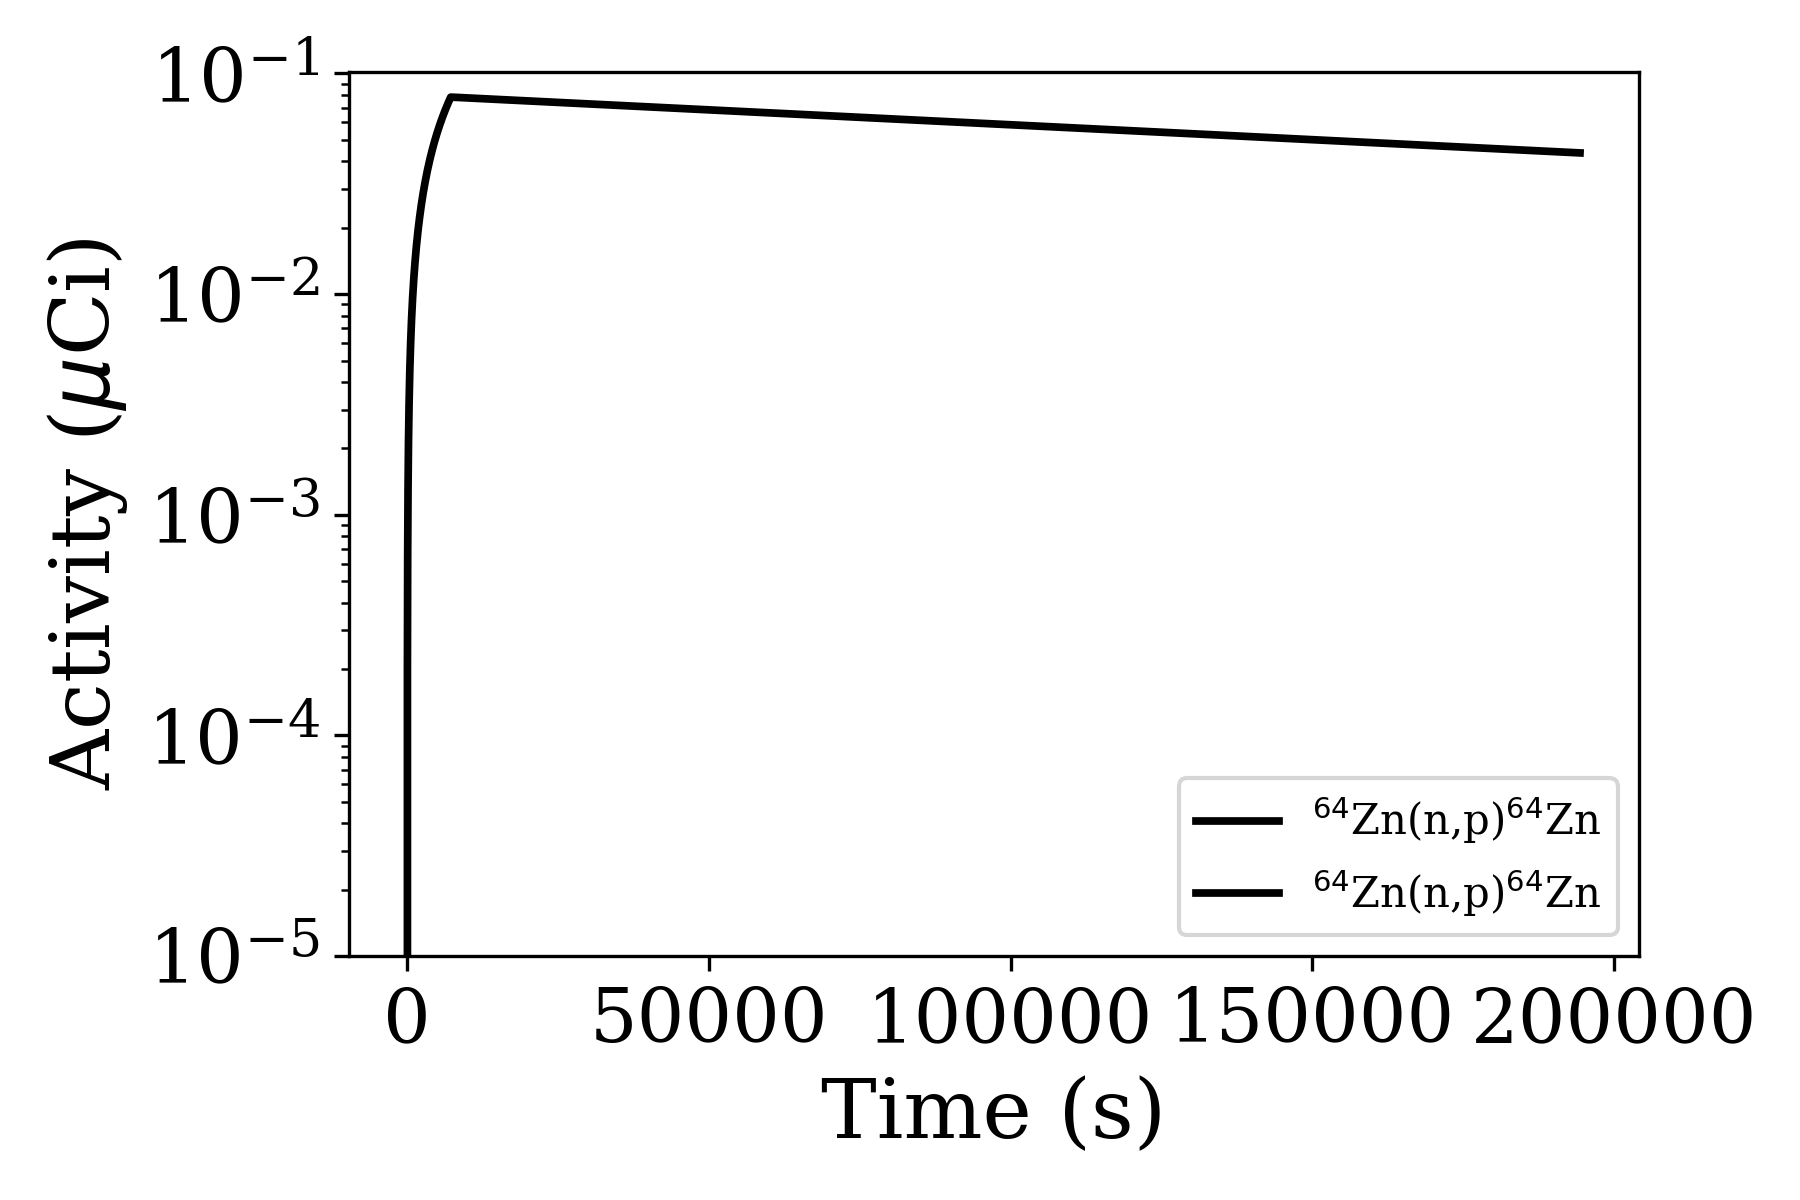
\includegraphics[width=.8\textwidth]{plot/Zn-64(n,p)Cu-64_wisconsin1} 

  \caption{A subfigure}
  \label{fig:sub1}
\end{subfigure}%
\begin{subfigure}{.5\textwidth}
  \centering
     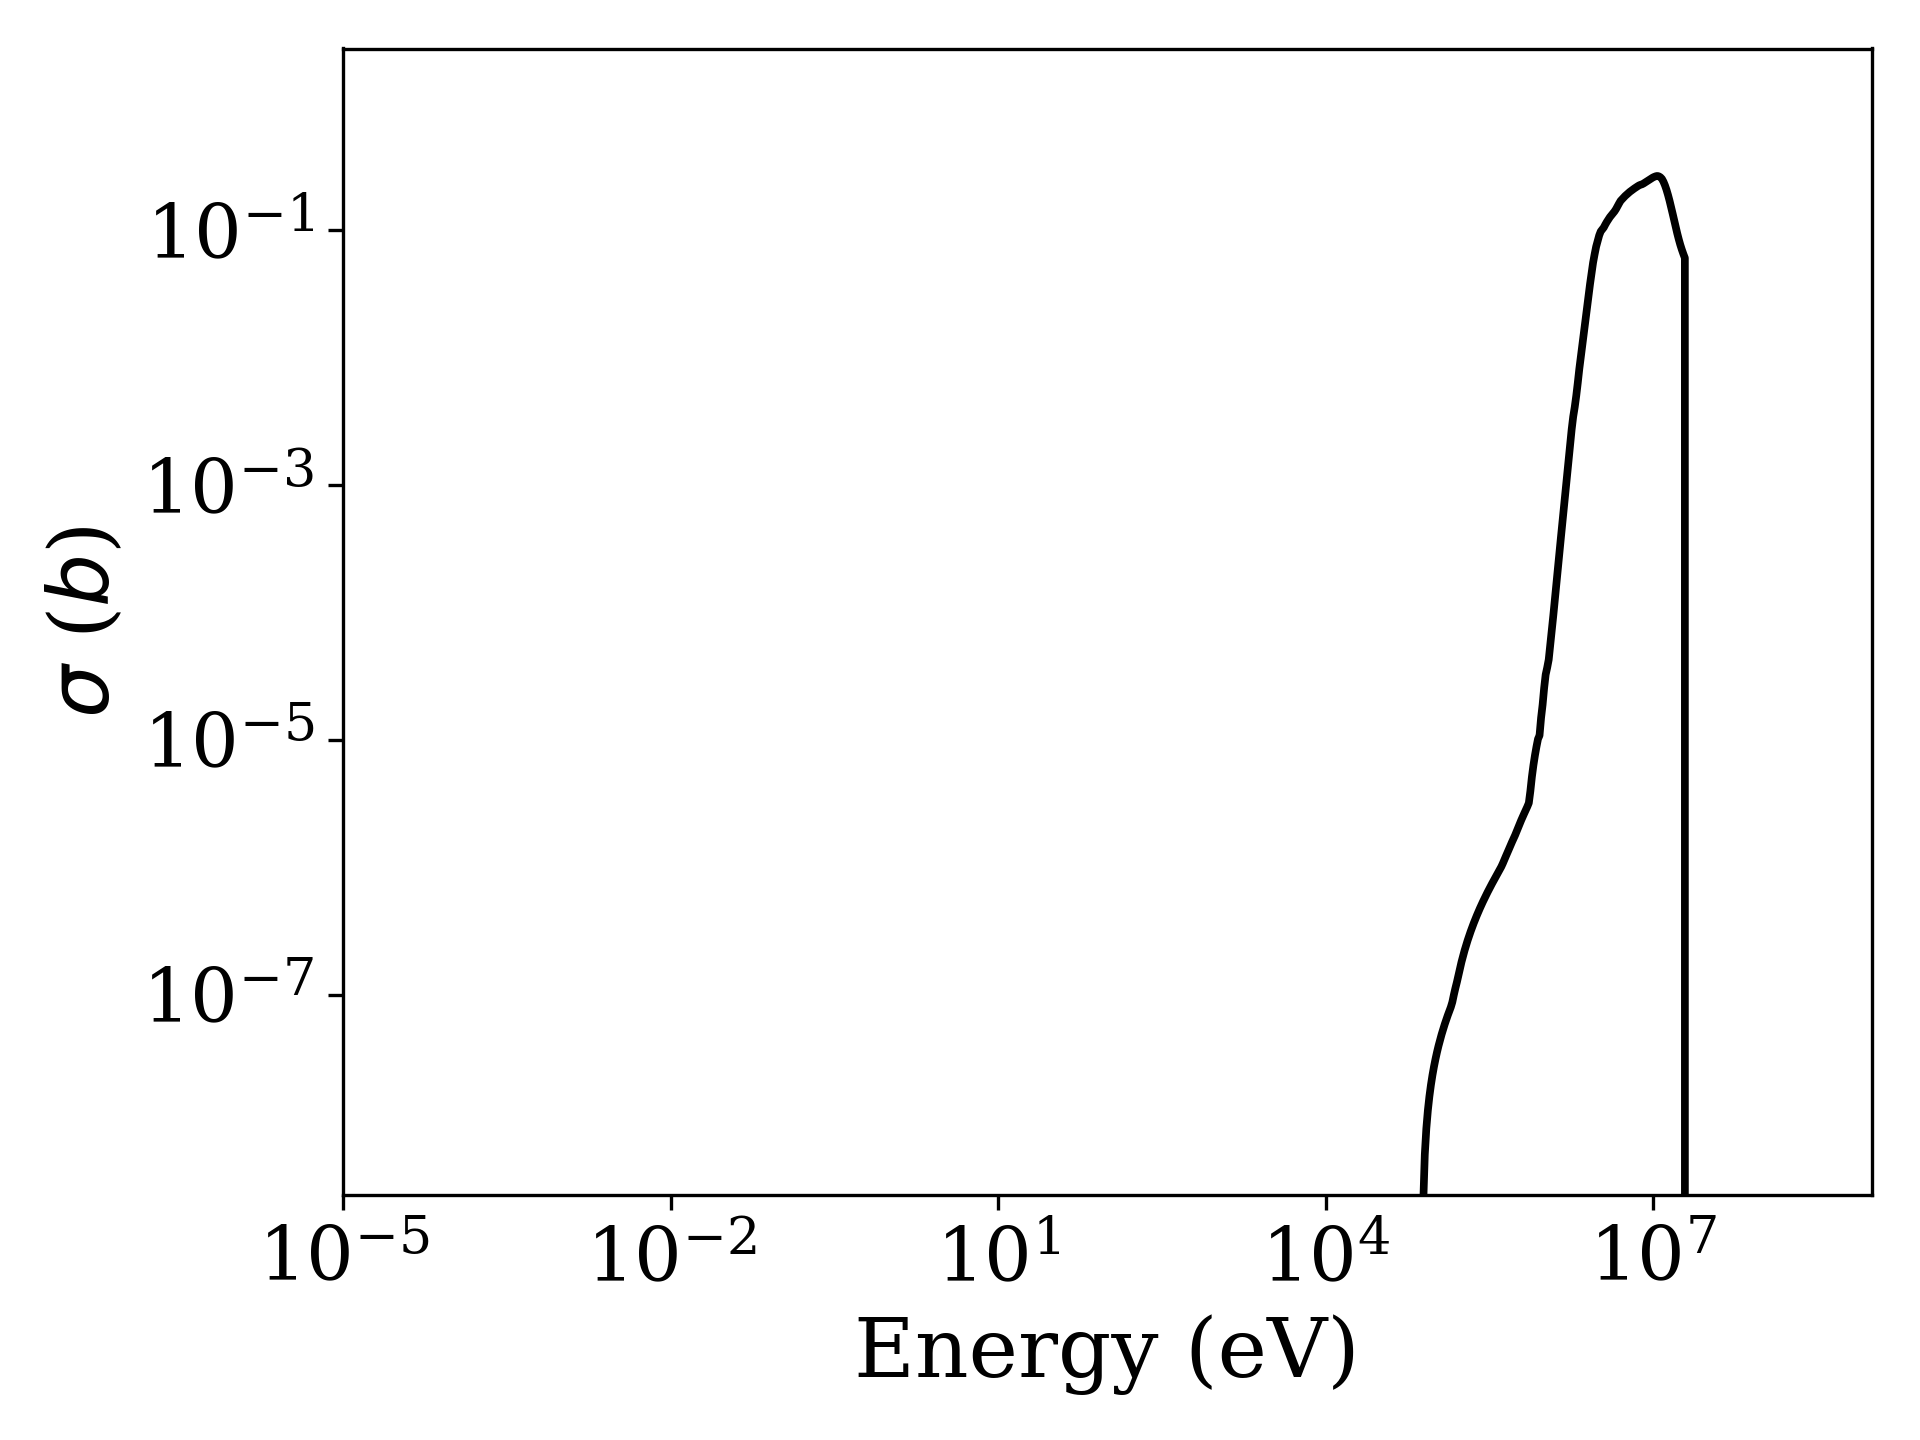
\includegraphics[width=.8\textwidth]{plot/Zn-64(n,p)Cu-64} 

  \caption{A subfigure}
  \label{fig:sub2}
\end{subfigure}
\caption{A figure with two subfigures}
\label{fig:test}
\end{figure}

\begin{table*}[h]
\centering
\begin{tabular}{ |c|c|c|c|c|c|c| }
 \hline
 Reaction & T$_{1/2}$ & ROI (eV) & Important Gammas (keV) \\
 \hline 
 $^{64}$Zn(n,p)$^{64}$Cu &  2.6 d & 2.47e+06, 8.16e+06 & 1345.77(0.00475) \\ 
\hline
\end{tabular}
\end{table*}
